%% Copernicus Publications Manuscript Preparation Template for LaTeX Submissions
%% ---------------------------------
%% This template should be used for copernicus.cls
%% The class file and some style files are bundled in the Copernicus Latex Package, which can be downloaded from the different journal webpages.
%% For further assistance please contact Copernicus Publications at: production@copernicus.org
%% https://publications.copernicus.org/for_authors/manuscript_preparation.html


%% Please use the following documentclass and journal abbreviations for preprints and final revised papers.

%% 2-column papers and preprints
\documentclass[journal abbreviation, manuscript]{copernicus}
%\documentclass[acp]{copernicus} % for some reason you have to run this a few times to get the abstract to appear


%% Journal abbreviations (please use the same for preprints and final revised papers)


% Advances in Geosciences (adgeo)
% Advances in Radio Science (ars)
% Advances in Science and Research (asr)
% Advances in Statistical Climatology, Meteorology and Oceanography (ascmo)
% Aerosol Research (ar)
% Annales Geophysicae (angeo)
% Archives Animal Breeding (aab)
% Atmospheric Chemistry and Physics (acp)
% Atmospheric Measurement Techniques (amt)
% Biogeosciences (bg)
% Climate of the Past (cp)
% DEUQUA Special Publications (deuquasp)
% Earth Surface Dynamics (esurf)
% Earth System Dynamics (esd)
% Earth System Science Data (essd)
% E&G Quaternary Science Journal (egqsj)
% EGUsphere (egusphere) | This is only for EGUsphere preprints submitted without relation to an EGU journal.
% European Journal of Mineralogy (ejm)
% Fossil Record (fr)
% Geochronology (gchron)
% Geographica Helvetica (gh)
% Geoscience Communication (gc)
% Geoscientific Instrumentation, Methods and Data Systems (gi)
% Geoscientific Model Development (gmd)
% History of Geo- and Space Sciences (hgss)
% Hydrology and Earth System Sciences (hess)
% Journal of Bone and Joint Infection (jbji)
% Journal of Micropalaeontology (jm)
% Journal of Sensors and Sensor Systems (jsss)
% Magnetic Resonance (mr)
% Mechanical Sciences (ms)
% Natural Hazards and Earth System Sciences (nhess)
% Nonlinear Processes in Geophysics (npg)
% Ocean Science (os)
% Polarforschung - Journal of the German Society for Polar Research (polf)
% Primate Biology (pb)
% Proceedings of the International Association of Hydrological Sciences (piahs)
% Safety of Nuclear Waste Disposal (sand)
% Scientific Drilling (sd)
% SOIL (soil)
% Solid Earth (se)
% State of the Planet (sp)
% The Cryosphere (tc)
% Weather and Climate Dynamics (wcd)
% Web Ecology (we)
% Wind Energy Science (wes)


%% \usepackage commands included in the copernicus.cls:
%\usepackage[german, english]{babel}
%\usepackage{tabularx}
%\usepackage{cancel}
%\usepackage{multirow}
%\usepackage{supertabular}
%\usepackage{algorithmic}
%\usepackage{algorithm}
%\usepackage{amsthm}
%\usepackage{float}
%\usepackage{subfig}
%\usepackage{rotating}
\usepackage{xcolor}
\usepackage{soul}
\usepackage{listings}
\usepackage{booktabs}


\begin{document}

\title{Idealized Particle-Resolved Large-Eddy Simulations to Evaluate the Impact of Emissions Spatial Heterogeneity on CCN Activity}

\Author[1]{Samuel}{Frederick}
\Author[2]{Matin}{Mohebalhojeh}
\Author[1,2]{Jeffrey}{Curtis}
\Author[2]{Matthew}{West}
\Author[1][nriemer@illinois.edu]{Nicole}{Riemer} %% correspondence author


\affil[1]{Department of Climate, Meteorology, and Atmospheric Sciences, University of Illinois Urbana--Champaign, 1301 W. Green St., Urbana, IL 61801, USA}
\affil[2]{Department of Mechanical Science and Engineering, University of Illinois Urbana--Champaign, 1206 W. Green St., Urbana, IL, 61801,USA}

%% If authors contributed equally, please mark the respective author names with an asterisk, e.g. "\Author[2,*]{Anton}{Smith}" and "\Author[3,*]{Bradley}{Miller}" and add a further affiliation: "\affil[*]{These authors contributed equally to this work.}".

\runningtitle{Impacts of Emissions SH on CCN activity}

\runningauthor{Frederick}

\received{}
\pubdiscuss{} %% only important for two-stage journals
\revised{}
\accepted{}
\published{}

%% These dates will be inserted by Copernicus Publications during the typesetting process.

\firstpage{1}

\maketitle

\begin{abstract}
Aerosol-cloud interactions remain a large source of uncertainty in global climate models (GCMs) due to complex, nonlinear processes that alter aerosol properties and the inability to represent the full compositional complexity of aerosol populations within large-scale modeling frameworks. The spatial resolution of GCMs is often coarser than the scale of the spatially varying emissions in the modeled geographic region. This results in diffuse, uniform concentration fields of primary aerosol and gas-phase species instead of spatially heterogeneous concentrations. Aerosol processes such as gas-particle partitioning and coagulation are concentration-dependent in a non-linear manner, and thus the representation of spatially heterogeneous emissions impacts aerosol aging and properties. This includes climate-relevant quantities key to aerosol-cloud interactions including particle hygroscopicity and cloud condensation nuclei (CCN) activity. We investigate the impact of emissions spatial heterogeneity on aerosol properties including CCN activity via a series of first-of-a-kind particle-resolved large-eddy simulations with the modeling framework WRF-PartMC-MOSAIC-LES. CCN concentrations within the planetary boundary layer (PBL) are compared across numerous scenarios ranging in emissions spatial heterogeneity. CCN concentrations at low supersaturations ($S=0.1\mbox{--}0.3\%$) increase in the upper PBL by up to 25\%
for emissions scenarios with high spatial heterogeneity when compared to a uniform emissions base case. Process level analysis indicates that this increase is due to enhanced nitrate formation among scenarios with high emissions spatial heterogeneity. 
\end{abstract}


%\copyrightstatement{TEXT} %% This section is optional and can be used for copyright transfers.


\introduction  %% \introduction[modified heading if necessary]

Aerosols exert a net negative radiative forcing, but significant
uncertainty remains in how aerosol-cloud interactions are represented
in climate models \citep{ipcc_report_2021}. Two major factors
contribute to this uncertainty: (1) the spatial resolution of models
and (2) the treatment of aerosol representation, which refers to how 
aerosol properties such as size distribution, chemical composition, 
and mixing state are modeled.

Advances in computational power have allowed modelers to investigate
how spatial resolution affects radiative forcing due to aerosol-cloud
interactions \citep{ma_how_2015}. At the same time, increasing
computational capabilities have enabled more sophisticated aerosol
representations \citep{zaveri_development_2021,
  tilmes_description_2023}. While both spatial resolution and aerosol
representation have advanced, they have largely been studied in
isolation. The combined effect of sub-grid scale spatial heterogeneity
and detailed aerosol representation on relevant properties, such as
cloud condensation nuclei (CCN) activity, remains largely unexplored.
The goal of this paper is to investigate their combined impact on key 
microphysical properties, with a focus on cloud condensation nuclei 
(CCN) activity.

Aerosol-aware climate models typically include a sub-model that
governs aerosol representation and associated processes. Due to
computational constraints, these aerosol treatments often simplify
compositional diversity. For instance, the Energy Exascale Earth
System Model (E3SM) uses the MAM4 scheme, which represents aerosols
using four internally mixed, lognormally distributed modes
\citep{golaz_doe_2022}. This approach inherently constrains the
diversity of aerosol populations, as all particles within a given mode
share identical composition. In reality, however, aerosols age
independently, leading to complex, highly heterogeneous
mixtures. Particle-resolved aerosol models address this limitation by
explicitly tracking the composition and evolution of individual
particles. The Particle Monte Carlo model (PartMC) \citep{riemer_simulating_2009} 
has been extensively used to study the sensitivity of
CCN activity to aerosol composition \citep{fierce_when_2013}, aging
timescales due to condensation and coagulation for carbonaceous CCN
\citep{fierce_explaining_2015}, and the impact of mixing state on CCN
estimates \citep{ching_metrics_2017}. Furthermore, PartMC has been
leveraged to quantify errors in CCN predictions from modal and
sectional models by comparing CCN concentrations against those derived
from fully resolved aerosol compositions
\citep{zaveri_particle-resolved_2010, ching_metrics_2017}. Comparisons
between PartMC and MAM4 have revealed substantial discrepancies in CCN
activity, particularly in polluted regions where coagulation and
gas-particle partitioning amplify model differences
\citep{fierce_quantifying_2024}.

Despite these advancements in aerosol representation, a critical gap
remains: the combined effects of high-resolution aerosol treatment and
fine-scale spatial heterogeneity have yet to be systematically
explored. Understanding this interaction is essential, as the
variability in surface properties, emissions, and resulting aerosol
plumes influences particle aging and CCN activity. The goal of this
study is to bridge this gap by conducting the first particle-resolved
large-eddy simulations (LES) to analyze how sub-grid scale spatial
heterogeneity affects aerosol composition, aging, and CCN activation.

Existing regional and global-scale aerosol-aware models lack the
resolution to fully capture fine-scale spatial heterogeneities,
leading to artificially uniform concentrations within grid cells. This
oversimplification distorts the representation of non-linear aerosol
processes such as coagulation and gas-particle partitioning. Studies
have demonstrated that climate-relevant aerosol properties, including
aerosol optical properties \citep{gustafson_jr_downscaling_2011} and
CCN activity \citep{weigum_effect_2016}, are highly sensitive to model
resolution. Much of the sub-grid scale variability arises from
spatially heterogeneous emissions \citep{qian_investigation_2010}, yet
many climate models fail to resolve this variability adequately.

Prior research on sub-grid variability of aerosol properties has
typically compared coarse-resolution global climate models (50--100 km)
against higher-resolution simulations (1--10 km)
\citep{qian_investigation_2010, gustafson_jr_downscaling_2011,
  weigum_effect_2016, crippa_impact_2017,
  lin_quantification_2017}. While increasing model resolution improves
the representation of emissions heterogeneities, unresolved spatial
variability persists at sub-kilometer scales. Additionally,
climate models rely on Reynolds-averaged Navier-Stokes
parameterizations to represent boundary-layer turbulence, which fail
to capture the full complexity of turbulent transport and its
influence on aerosol processes.

Another approach to investigating sub-grid heterogeneity has been to use
LES, which explicitly captures fine-scale turbulent mixing and
chemical segregation.  \citet{brasseur_segregation_2023} review LES
applications investigating turbulence-chemistry interactions in
spatially heterogeneous environments.  Many LES studies have focused
on gas-phase chemistry, particularly the oxidation of reactive
volatile organic compounds (VOCs) such as isoprene, demonstrating that
spatially heterogeneous emissions contribute to chemical segregation
between reactive species in the boundary layer
\citep{ouwersloot_segregation_2011, kaser_chemistry-turbulence_2015}.
Given the coupling between gas and aerosol phases through gas-particle
partitioning, it is likely that chemical segregation due to spatially
heterogeneous emissions also influences aerosol properties. While some
LES-based studies have incorporated aerosols, they have largely relied
on simplified treatments. Recent efforts have coupled
turbulence-resolving frameworks with aerosol models, such as the
Sectional Aerosol Model for Large Scale Applications (SALSA)
\citep{kokkola_salsa_2008} with UCLALES
\citep{tonttila_uclalessalsa_2017} as well as the Parallelized Large-Eddy
Simulation Model (PALM) \citep{kurppa_implementation_2019}. Additional efforts coupling LES with prognostic aerosol treatments include the modal aerosol model M7 \citep{vignati_m7_2004} with the Dutch Atmospheric Large-Eddy Simulation model (DALES)
\citep{de_bruine_explicit_2019}. However, despite their
high-resolution transport schemes, these models rely on relatively
coarse aerosol representations. For example, UCLALES-SALSA employs a
10-bin sectional scheme, while DALES modifies the seven-mode M7 model
to incorporate additional hydrometeor modes. To our knowledge, no
turbulence-resolving model has yet incorporated a particle-resolved
aerosol treatment, which would enable a fully detailed representation
of aerosol composition, properties, and aging alongside LES-resolved
turbulent transport.

This study aims to analyze the coupled effects of spatial
heterogeneity in surface emissions (including both gas-phase species
and primary aerosols), aerosol aging processes, and their impact on
CCN activity. To achieve this, we conduct the first particle-resolved
LES simulations, establishing a high-resolution aerosol-transport
modeling framework that explicitly represents both turbulent transport
and aerosol composition.

This paper is organized in the following manner. Section \ref{methods}
presents the modeling framework, WRF-PartMC-MOSAIC-LES, along with a
description of emissions scenarios with varying spatial
heterogeneity. Section \ref{results} discusses the results of simulation runs,
including changes in aerosol size distribution, composition,
hygroscopicity, and CCN activity. We conclude with remarks on the
implications of this study, limitations stemming from its idealized
nature, and potential directions for future work.

\section{Methods}\label{methods}

\subsection{WRF-PartMC-MOSAIC-LES}

The aerosol-transport model WRF-PartMC-MOSAIC-LES integrates multiple
sub-models responsible for transport, aerosol representation, and
multiphase chemistry. It is extends the aerosol-transport column model
WRF-PartMC, originally developed by \citet{curtis_single-column_2017}
and later extended to include advection
\citep{gmd-17-8399-2024}. WRF-PartMC couples the Weather Research and
Forecasting model (WRF) \citep{skamarock_description_2008} with the
particle-resolved aerosol model PartMC
\citep{riemer_simulating_2009}. PartMC represents a population of
aerosol particles using an ensemble of computational particles, each
assigned a weight (i.e., particle multiplicity) to capture the
diversity of particle sizes and composition observed in real-world
aerosol populations. As particles age, their composition evolves
dynamically. Since PartMC operates as a box model it does not track
the spatial position of individual particles within a computational
grid cell. Instead, particle transport is handled by a stochastic
advection algorithm that interfaces with WRF's dynamical core
\citep{gmd-17-8399-2024}. WRF-PartMC has been used in one-dimensional
simulations to resolve vertical gradients in aerosol composition and
mixing state \citep {curtis_single-column_2017} and, more recently, in
three-dimensional simulations to study aerosol transport within a
regional domain driven by by simulated meteorology
\citep{gmd-17-8399-2024}.

LES models explicitly resolve large-scale turbulent motion, typically
at the scale of 10--100~m; however, they must parameterize sub-grid
scale eddies and the down-gradient tendency of turbulent kinetic
energy (TKE) as it propagates from large to small scales, where it
ultimately dissipates as heat. This requires the use of closure
schemes. In WRF-PartMC-MOSAIC-LES, turbulent mixing is parameterized
using Deardorff's TKE scheme for eddy diffusivity and eddy viscosity
\citep{deardorff_stratocumulus-capped_1980}.

Gas-phase chemistry, gas-aerosol partitioning, and aerosol
thermodynamics are represented using the Model for Simulating Aerosol
Interactions and Chemistry (MOSAIC) \citep{zaveri_model_2008}. MOSAIC
is comprised of multiple sub-models, including the Carbon Bond
Mechanism version Z (CBM-Z) which solves gas phase chemistry
\citep{zaveri_new_1999}. Phase-dependent partitioning of aerosol
species is handled by the Multicomponent Equilibrium Solver for
Aerosols (MESA) \citep{zaveri_computationally_2005}. Activity
coefficients of electrolytes are parameterized via the Multicomponent
Taylor Expansion Method (MTEM) \citep{zaveri_new_2005}. To efficiently
solve the numerically stiff set of solid-liquid phase reactions,
MOSAIC employs the Adaptive Step Time-Split Euler Method (ASTEM)
\citep{zaveri_model_2008}. MOSAIC models aerosol chemistry for both
inorganic and organic compounds such as nitrate, ammonium, sulfate,
black carbon (BC), and a limited set of secondary organic aerosol
(SOA) species.

\subsection{Computational domain setup}

The computational domain extends 10~km in both the $x$- and
$y$-directions, with a horizontal grid spacing of 100~m.  Vertically,
the domain reaches 2~km and is represented with 200~vertical
levels. LES runs in WRF use an $\eta$ vertical coordinate system,
whereby vertical levels are linearly spaced in pressure. Due to the
limited depth of the domain, this results in an effective vertical
resolution of approximately 10~m. Simulations begin on the Vernal
Equinox at 09:00~local time (LT) and conclude at 15:00~LT for a total
duration of 6~hours to maintain balanced photolysis rates throughout
the simulation period. Each grid cell is initialized with
100~computational particles, resulting in 100~million total
particles. As processes such as emission, transport, and coagulation
modify the number concentration of particles, the total number of
computational particles within each grid cell is dynamically
adjusted---doubling when it falls to half the initial value and
halving when it reaches twice the initial value---to maintain
computational efficiency and adequate representation of the aerosol
state. 
\textcolor{blue}{Customarily, the number of computational particles $N_{\mathrm{p}}$ per grid cell is set around $N_{\mathrm{p}} = 10,000$ as stochastic error in processes such as advection decreases according to $1/\sqrt{N_{\mathrm{p}}}$ \citep{gmd-17-8399-2024}. However, computational demand grows with $N_{\mathrm{p}}$, placing constraints on our ability to increase the number of particles. Simulations in this paper were conducted on a high-performance computing cluster with 384 CPU cores executing in parallel.}

\textcolor{red}{We want to have something that conveys that we still
  can trust the results (I hope??). I suggest this, what do you think?
  We In particle-resolved box model studies, a typical choice is
  $N_{\mathrm{p}} \sim 10{,}000$ computational particles to minimize
  stochastic variability in aerosol processes
  \citep{gmd-17-8399-2024}[maybe better would be to cite actual box
    model studies, for example Yicen's paper].  However, for
  three-dimensional large-eddy simulations (LES) coupled with PartMC,
  the computational burden scales with the number of grid cells,
  making such high particle counts per cell impractical. In this
  study, we used 100 particles per grid cell—a choice that balances
  computational cost and model fidelity. While lower $N_{\mathrm{p}}$
  increases stochastic variability at the individual grid-cell level,
  our focus is on domain-scale patterns and contrasts driven by
  spatial heterogeneity, which are robust to such noise. Simulations
  were conducted on a high-performance computing cluster using 384 CPU
  cores in parallel. Future studies may explore sensitivity to
  $N_{\mathrm{p}}$, but we expect the main conclusions presented here
  to remain valid.}


  In
  contrast, for three-dimensional large-eddy simulations (LES) coupled
  with PartMC, the computational burden scales with the number of grid
  cells, making such high particle numbers per cell impractical. In
  this study, we used 100 particles per grid cell—sufficient to
  resolve the key aerosol processes while enabling domain-wide
  coupling with turbulence over a six-hour simulation period. While
  this lower $N_{\mathrm{p}}$ increases stochastic variability at the
  individual grid-cell level, our focus is on domain-scale patterns
  and contrasts driven by spatial heterogeneity, which are robust to
  particle noise. All simulations were performed on a high-performance
  computing cluster using 384 CPU cores in parallel. Future studies
  may explore higher particle counts in targeted regions or
  sensitivity runs, but we expect the main conclusions of this study
  to hold.}

The domain is initialized over a flat, uniform land surface absent of
topographic features or land-use variations. WRF-PartMC-MOSAIC-LES is
not coupled to one of WRF's radiation sub-models. Instead, MOSAIC
employs idealized parameterizations to determine photolysis rates
based on the solar zenith angle. Due to the lack of a radiation
sub-model, surface heating is imposed uniformly across the domain
using a constant rate of 0.24~$\rm K \, m \, s^{-1}$, which is
representative of typical kinematic heat fluxes observed during
mid-day in clear sky conditions over land
\citep{stull_introduction_1988}. %Ch. 7 S 7.1, pg. 252
\textcolor{red}{When citing a book, it's great to include the
  chapter/section.}

Initial conditions and emissions for both aerosols and the gas phase
represent an urban environment and are based on
\citet{riemer_simulating_2009}. The initial concentrations and
emission rates stem from the 1987 Southern California Air Quality
Study (SCAQS), which collected measurements of gas phase species and
particulate matter mass concentrations at multiple sites across the
Los Angeles basin \citep{zaveri_model_2008}. Table
\ref{table:gas_emiss_ics} provides initial concentrations and emission
rates for gas phase species, while Table \ref{table:aero_emiss_ics}
details aerosol initial conditions and emission rates categorized by
aerosol modes. Initially, the aerosol consists of an internal mixture
composed of 50\% ammonium sulfate and 50\% primary organic aerosol
(POA) by mass.  The three emission modes representing cooking and
vehicular combustion comprise varying mixtures of POA and BC. The
three emission modes, representing cooking and vehicular combustion
sources, each consist of distinct fixed mixtures of primary organic
aerosol (POA) and black carbon (BC). To allow for simulation spin-up
and the full development of the convective boundary layer, emissions
remain at zero during the first hour of simulation. Subsequently,
surface emissions are released at constant rates as specified by
Tables \ref{table:gas_emiss_ics} and \ref{table:aero_emiss_ics} for
the remainder of simulations.


\begin{table}[!t]
\centering
\caption{Gas phase emissions and initial conditions. Table adapted from \citet{riemer_simulating_2009} with permission.}
\begin{tabular*}{\linewidth}{@{\extracolsep{\fill}} lccr}
\\[-2ex]\hline 
     \hline \\[-2ex] Species & Symbol & Initial Mole Fraction (ppb) & Emissions (nmol m\textsuperscript{-2} s\textsuperscript{-1}) \\
\midrule
Nitric oxide & NO & 0.1 & 31.8 \\
Nitrogen dioxide & NO\textsubscript{2} & 1.0 & 1.67 \\
Nitric acid & HNO\textsubscript{3} & 1.0 & \\
Ozone & O\textsubscript{3} & 50.0 & \\
Hydrogen peroxide & H\textsubscript{2}O\textsubscript{2} & 1.1 & \\
Carbon monoxide & CO & 21 & 291.3 \\
Sulfur dioxide & SO\textsubscript{2} & 0.8 & 2.51 \\
Ammonia & NH\textsubscript{3} & 0.5 & 6.11 \\
Hydrogen chloride & HCl & 0.7 & \\
Methane & CH\textsubscript{4} & 2200 & \\
Ethane & C\textsubscript{2}H\textsubscript{6} & 1.0 & \\
Formaldehyde & HCHO & 1.2 & 1.68 \\
Methanol & CH\textsubscript{3}OH & 0.12 & 0.28 \\
Methyl hydrogen peroxide & CH\textsubscript{3}OOH & 0.5 & \\
Acetaldehyde & ALD2 & 1.0 & 0.68 \\
Paraffin carbon & PAR & 2.0 & 96 \\
Acetone & AONE & 1.0 & 1.23 \\
Ethene & ETH & 0.2 & 7.2 \\
Terminal olefin carbons & OLET & 2.3 \(\cdot 10^{-2}\) & 2.42 \\
Internal olefin carbons & OLEI & 3.1 \(\cdot 10^{-4}\) & 2.42 \\
Toluene & TOL & 0.1 & 4.04 \\
Xylene & XYL & 0.1 & 2.41 \\
Lumped organic nitrate & ONIT & 0.1 & \\
Peroxyacetyl nitrate & PAN & 0.8 & \\
Higher organic acid & RCOOH & 0.2 & \\
Higher organic peroxide & ROOH & 2.5 \(\cdot 10^{-2}\) & \\
Isoprene & ISOP & 0.5 & 0.23 \\
Alcohols & ANOL & & 3.45 \\
\\[-2ex]\hline 
     \hline \\[-2ex]
\end{tabular*}
\label{table:gas_emiss_ics}
\end{table}


\begin{table}[!t]
\centering
\caption{Aerosol emissions and initial conditions. Table adapted from \citet{riemer_simulating_2009} with permission.}
\begin{tabular*}{\linewidth}{@{\extracolsep{\fill}} cccccc}
\\[-2ex]\hline 
     \hline \\[-2ex] Initial/Background  & $N$ (m$^{-3}$) & $D_{\text{gn}}$ ($\mu$m) & $\sigma_g$ & Composition by Mass\\
 \midrule
Aitken Mode & $3.2 \cdot 10^9$ & 0.02 & 1.45 & 50\% (NH$_4$)$_2$SO$_4$, 50\% POA\\
Accumulation Mode & $2.9 \cdot 10^9$ & 0.116 & 1.65 & 50\% (NH$_4$)$_2$SO$_4$, 50\% POA\\
\midrule
Emissions & $E$ (m$^{-2}$ s$^{-1}$) & $D_{\text{gn}}$ ($\mu$m) & $\sigma_g$ & Composition by Mass\\
\midrule
Meat cooking & $9 \cdot 10^6$ & 0.086 & 1.9 & 100\% POA\\
Diesel vehicles & $1.6 \cdot 10^8$ & 0.05 & 1.7 & 30\% POA, 70\% BC \\
Gasoline vehicles & $5 \cdot 10^7$ & 0.05 & 1.7 & 80\% POA, 20\% BC \\
\\[-2ex]\hline 
     \hline \\[-2ex]
\end{tabular*}
\label{table:aero_emiss_ics}
\end{table}

Meteorological initial conditions define an idealized
convective boundary layer structure, where the surface is 5~K warmer
than the mixing layer, and an inversion of 8~K caps the layer at 1
km. The wind profile is set to zero throughout the domain.
%\hl{Maybe include a figure here?}  

%\hl{putting some namelist parameters here for time being for convenience}
%\begin{lstlisting}
% &physics
% mp_physics                          = 0,     0,     0, ! microphysics scheme
% ra_lw_physics                       = 0,     0,     0, ! long wave radiation scheme
% ra_sw_physics                       = 0,     0,     0, ! short wave radiation scheme
% radt                                = 0,     0,     0, ! radiation time step
% sf_sfclay_physics                   = 0,     1,     1, ! surface layer parameterization
% sf_surface_physics                  = 0,     0,     0, ! surface sub model
% bl_pbl_physics                      = 0,     0,     0, ! boundary layer parameterizations
% bldt                                = 0,     0,     0, !  boundary layer scheme time delta
% cu_physics                          = 0,     0,     0, ! cumulus physics model
% cudt                                = 0,     0,     0, ! cumulus physics scheme time delta
% isfflx                              = 2, ! surface heat and moisture flux
% num_land_cat = 24,
% num_soil_layers                     = 5, ! does this matter since I don't use a surface model?
%\end{lstlisting}


\subsection{Emissions Scenarios}

\begin{figure}[!t]
	\centering
	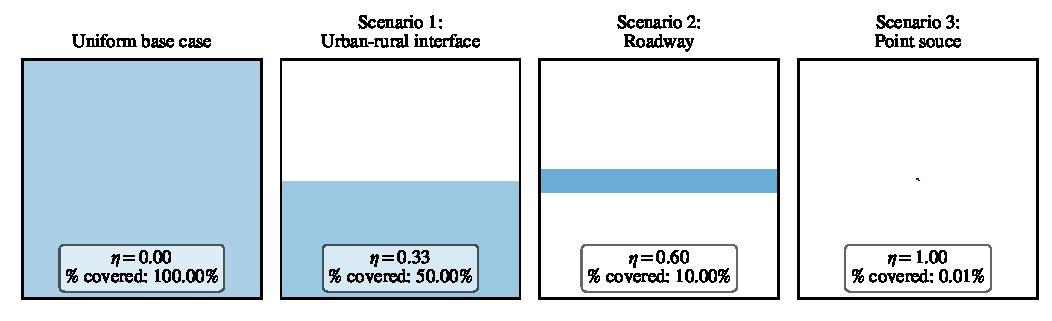
\includegraphics[]{figures/SH-scenarios.pdf}
	\caption{Emissions spatial heterogeneity scenarios. The
          pattern of emissions is shown as a cross section of the
          $x$-$y$ plane at ground level. Shaded areas correspond to
          regions of emissions. The hue of shading indicates the
          intensity of emissions scaling ranging from light blue (low
          emissions scaling) to dark blue (high emissions
          scaling). Both the spatial heterogeneity metric $\eta$ and
          the fraction of area covered by emissions are displayed in
          the bottom of each scenario.}
	\label{fig:sh-scenarios}
\end{figure} 

To assess the impact of emissions spatial heterogeneity on aerosol
properties, we examine multiple emissions scenarios, shown in Figure
\ref{fig:sh-scenarios}. The first scenario, referred to as the uniform
base case, distributes emissions evenly across the entire domain. This
serves as a proxy for coarser-resolution models that do not resolve
spatial heterogeneity of emissions and instead assume uniform
emissions of gases and primary aerosols across grid cells. The
remaining scenarios introduce increasing levels of spatial
heterogeneity, enabling direct comparison against the uniform base
case to evaluate a scenario's influence on aerosol properties. Scenario~1
represents an idealized urban-rural interface, where emissions are
released in half the domain with no emissions occurring in the other
half. Scenario~2 contains a narrow strip of emissions running through
the center of the domain, corresponding to an emission pattern typical
of a major roadway. Lastly, Scenario~3 places all emissions in a
single grid cell in the domain center representing a point source such
as an industrial plume.

These scenarios span a range of spatial heterogeneity, which is
quantified using the metric $\eta$ developed by
\citep{mohebalhojeh_2024} \hl{make sure to update this citation when
  Matin's paper is published}. The metric $\eta$ is a normalized
measure of spatial heterogeneity, ranging from 0 (completely
homogeneous) to 1 (maximally heterogeneous). For a discrete
2-dimensional scalar field $f$ over a domain $S$ with lateral
dimensions $N$ by $M$, $\eta$ is defined as

\begin{equation}
\eta(f, S) = \frac{\sum_{\tilde{S}\in \mathbb{R}}|\overline{f}(S) - \overline{f}(\tilde{S})|}{\overline{f}(S)\left[\frac{3}{2}(N\times M)(N-1)(M-1) + N(N-1) + M(M-1)\right]}, 
\end{equation}
where $\overline{f}(S)$ is the domain mean and
$\overline{f}(\tilde{S})$ is the mean over a subset of the domain
$\tilde{S}$. Thus, the metric is computed by summing the absolute
value of the difference between the domain mean $\overline{f}(S)$ and
all domain subset means $\overline{f}(\tilde{S})$, normalized by the
product of the domain mean and the number of possible
subsets. \citet{mohebalhojeh_2024} show that the metric is
translationally invariant when the scalar field $f$ is shifted within
$S$. Furthermore, they prove that the
maximum spatial heterogeneity occurs when the
scalar field is zero everywhere except at a single point
where it takes the value $MN\times\overline{f}(S)$.

Thus, the uniform base case corresponds to the homogeneous condition
($\eta = 0$) while Scenario~3---the point-source
emission---represents the maximally heterogeneous case ($\eta =
1$). To ensure consistent mass emissions across scenarios, emission
rates are scaled by the fraction of area covered by emissions. For
instance, in Scenario~3, this results in a scaling of $10,000$
($M=N=100$) for the point-source emission. The fraction of area
covered by emissions is displayed for each scenario alongside the
spatial heterogeneity values in Figure \ref{fig:sh-scenarios}.

\section{Results}\label{results}

Key findings of this paper are structured as follows. Section
\ref{sec:gas-impacts} investigates the relationship between emissions
spatial heterogeneity and the gas phase. Section \ref{sec:size-dist}
presents impacts of emissions spatial heterogeneity on bulk aerosol
properties (number and mass concentrations). Section
\ref{sec:aero-comp} discusses impacts on aerosol composition, with
particular focus on sulfate, ammonium, and nitrate due to their
important role in particle hygroscopicity. Leveraging the
particle-resolved framework, we further evaluate how particle
hygroscopicity responds to emissions spatial heterogeneity. Building
on these results, Section \ref{sec:ccn-activ} investigates how
emissions spatial heterogeneity impacts CCN activity across a range of
supersaturation levels ranging ($0.1\%$ to $1.0\%$). Lastly, we
explore the governing role of aerosol composition--namely, the
presence of ammonia---in mediating the impact of emissions spatial
heterogeneity on CCN activity.

\subsection{Impacts of emissions spatial heterogeneity on gas phase species}\label{sec:gas-impacts}

\begin{figure}[!h]
	\centering
	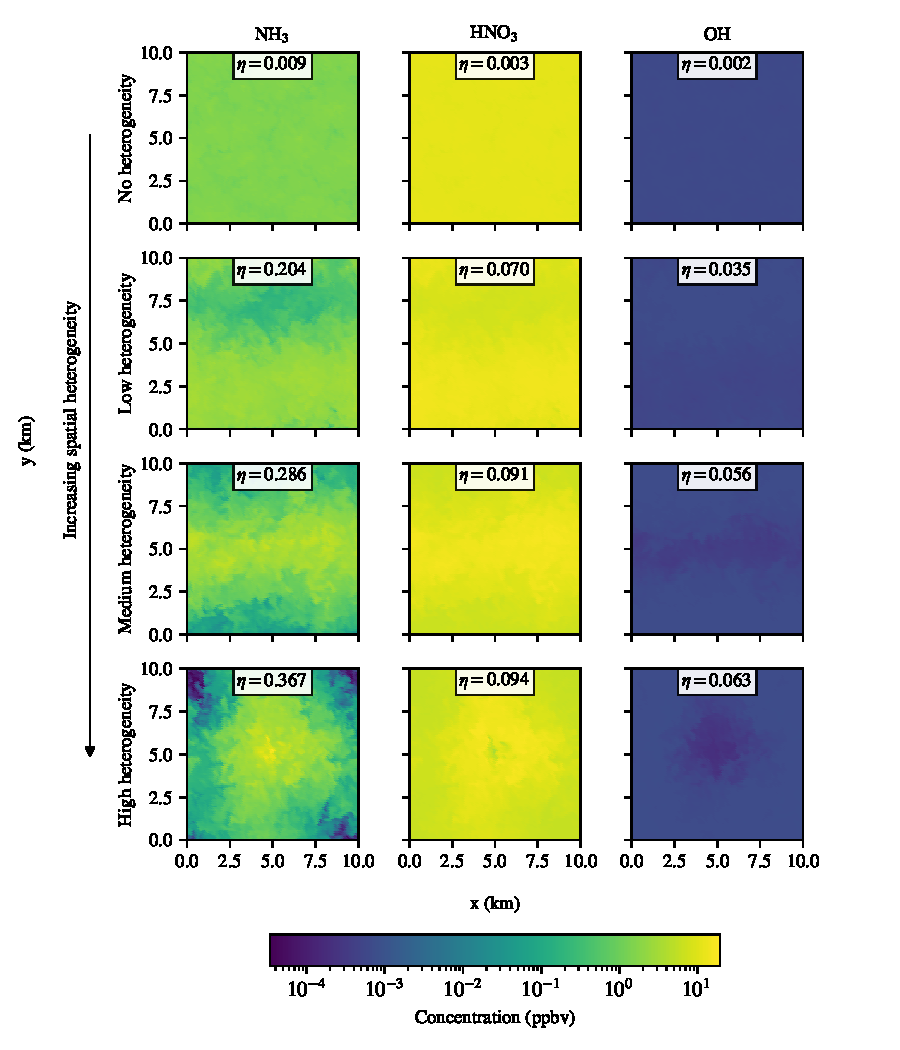
\includegraphics[]{figures/gas-spatial-heterogeneity-time36-z45.pdf}
	\caption{Cross sections in the $x$-$y$ plane of gas phase
          species NH$_3$ (left column), HNO$_3$ (center column), and
          OH (right column). Cross sections are shown at a height of
          approximately $z\approx900$ m and at $t=6$~h. Coloring
          indicates the concentration of gas species in parts per
          billion by volume. The value of the spatial heterogeneity
          metric $\eta$ is displayed alongside each cross section
          plot.}
	\label{fig:gas-cross-sec}
\end{figure} 

Figure \ref{fig:gas-cross-sec} displays $x$-$y$ cross sections of
ammonia, nitric acid, and the hydroxyl radical (OH) at $t=6$~h taken
at $z\approx900$~m in the upper boundary layer. Among the three
species, ammonia exhibits the highest spatial heterogeneity with
$\eta$ values 3--4 times higher than those of nitric acid and OH. This
is primarily because ammonia is emitted while nitric acid and OH are
formed due to chemical reactions. This leads to a marked concentration
gradient for ammonia between regions near the emissions plume (in
excess of 10~ppbv directly over the emissions plume in Scenario~3) and
farther toward the perimeter of the domain (as low as 0.1~pptv).

\textcolor{red}{This still needs to be revised. HNO3 and OH actually
  behave very similarly in terms of SH, NH3 has a larger SH, we think
  this is because NH3 is directly emitted...}  The similar structure
between ammonia and nitric acid indicates that nitric acid formation
is most effective over the emissions plume due to the emission of NO
and NO$_2$. The spatial pattern of OH follows that of ammonia and
nitric acid but with an inverse relationship: OH concentrations are
lower near the center of the emissions plume and higher concentrations
farther away. This indicates rapid oxidation of many reactive
compounds occurring in the emissions plume. Consequently, OH becomes
spatially segregated from its reactants in the emissions plume as OH
in the immediate vicinity of the plume is consumed.

The spatial heterogeneity of these compounds is further controlled by
the relative importance of turbulence in mixing reactive compounds and
their chemical reactivity. This relationship is characterized via the
Damköhler number, which is the ratio of the turbulent and chemical
reaction timescales,

\begin{equation}
D_a = \frac{\tau_{\mathrm{turb}}}{\tau_{\mathrm{chem}}}.
\end{equation}

When the chemical reaction timescale is shorter than the turbulent
timescale, such as in fast reactions including the production of OH
and its oxidation of other compounds, $D_a > 1$ such that the
concentration of OH is controlled by the turbulent timescale. As a
result, local concentrations of OH are in near chemical-equilibrium as
it is produced and consumed over very short timescales, preventing
large scale spatial heterogeneity in the domain-wide concentration of
OH. Conversely, compounds such as ammonia and nitric acid undergo
comparatively slower chemical reactions, whereby $D_a < 1$, indicating
that the rate of chemical reaction determines the abundance of
reactants and products. This allows for the build-up of stronger
concentration gradients between the emissions plume and the
surrounding region. The absence of vertical wind shear within
simulations limits the strength of shear-induced turbulence and
horizontal mixing, resulting in substantial concentration gradients
away from the emissions plume for ammonia and nitric acid.


\begin{figure}[!h]
	\centering
	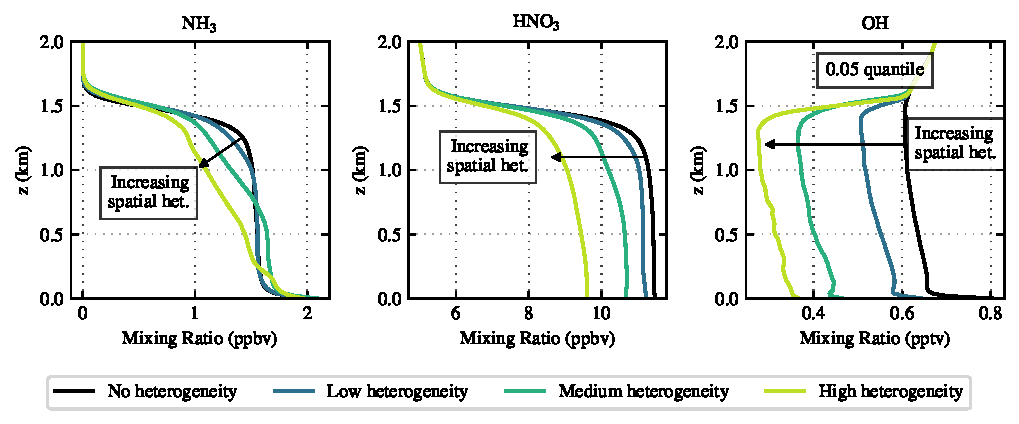
\includegraphics[]{figures/aerosol-gas-vertical-profiles-time36.pdf}
	\caption{Vertical profiles of gas phase species NH$_3$ (left),
          HNO$_3$ (center), and OH (right) at $t=6$~h. For NH$_3$
          (left) and HNO$_3$, the mean value is displayed at each
          vertical level. For OH, the 5th percentile at each vertical
          level is shown to indicate the local changes to the OH
          concentration near the emissions plume. Values for the
          uniform base case are shown as a solid black line while
          emissions scenarios 1--3 are shown as colored solid lines.}
	\label{fig:gas-profiles}
\end{figure} 

Figure \ref{fig:gas-profiles} presents vertical profiles of ammonia,
nitric acid, and OH. For ammonia and nitric acid, the profiles show
horizontal averages at each vertical level across the entire domain.
As emissions spatial heterogeneity increases, both ammonia and nitric
acid concentrations decrease on average. As will demonstrated in
Section \ref{sec:aero-comp}, this is due to increased partitioning of
these species into the aerosol phase to form ammonium nitrate.

For OH, the vertical profiles show the 5th percentile of
concentrations within each level, rather than the domain-wise mean, to
better capture localized depletion near the emissions plume. Scenarios
with high emissions spatial heterogeneity result a pronounced
reduction in OH near the emissions plume. Whereas in the uniform base
case, the level-mean concentration of OH is 0.61~pptv at $z=1$~km,
whereas in Scenario~3 they drop by 54\%
to 0.28~pptv.

\subsection{Aerosol size distributions}\label{sec:size-dist}

\begin{figure}[!h]
	\centering
	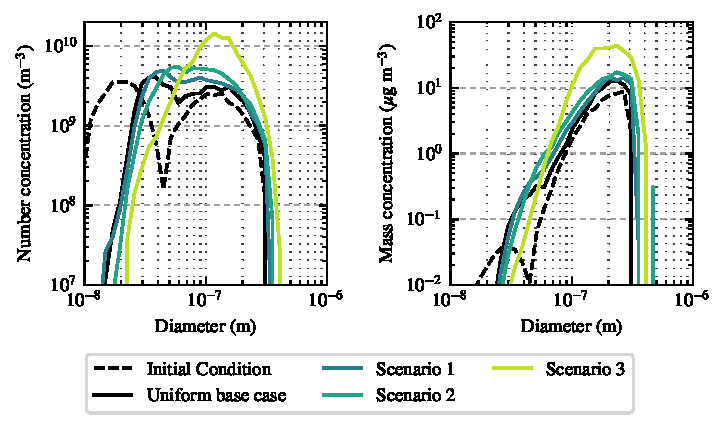
\includegraphics[]{figures/combined_num_mass_conc_i50_j50_k60.pdf}
	\caption{Number (left) and mass (right) distributions for each emissions scenario in the upper boundary layer ($z=800$)~m and $t=6$~h. The initial condition is shown as the dashed black line. Values for the uniform base case are shown as a solid black line while emissions scenarios 1--3 are shown as colored solid lines.}
	\label{fig:size-dists}
\end{figure} 

Number and mass distributions for each emissions scenario are shown in
Figure \ref{fig:size-dists}. Each size distribution is taken from a
vertical level in the upper boundary layer at $z\approx800$ m. When
analyzing size distributions for a single grid cell, considerable
stochastic noise is present in the shape of distributions. This is due
to the selected number of computational particles per grid cell ($N =
100$) alongside the stochastic treatment of aerosol particles in
WRF-PartMC. To reduce stochastic noise, number and mass distributions
represent the average distribution in a 1~km$^2$ region centered over
the emissions plume (i.e., size distributions are averaged over a
$10\times10$ grid cell region). For the uniform base case, Scenario~2
and Scenario~3, this region is directly over the center of the
domain. For Scenario~1, emissions are released in one half of the
domain that is offset from the center, and thus the averaging region
is located in the center of the emissions patch. For each size
distribution, data have been binned into 100 logarithmically spaced
bins, ranging in size from $10^{-9}$ to $10^{-3}$~m.

To quantify changes in particle populations, the number and mass
concentration of Aitken ($D_{\rm p} \leq 50$~nm) and accumulation
($D_{\rm p} > 50$~nm) mode particles were calculated. As the spatial
heterogeneity of emissions increases, the number of Aitken mode
particles decreases by up to 81\% while the number of accumulation
mode particles increases by up to 246\%. The decrease in Aitken mode
particles is attributable to enhanced Brownian coagulation due to
higher local concentrations near the emissions plume core. The
corresponding increase in accumulation mode particles is a result of
secondary aerosol formation.  Changes to aerosol composition due to
gas-particle partitioning is explored in further detail in the next
section.

Similarly, the mass distribution of Aitken mode particles decreases by
up to 74\% for high emissions spatial heterogeneity scenarios, while
the accumulation mode mass fraction increases by up to
309\%. Coagulation of smaller Aitken mode particles with accumulation
mode particles contributes little change in the mass distribution as
indicated by a slight reduction in the Aitken mode mass
concentration. Alongside the increase in the number of accumulation mode 
particles, the increase in mass concentration among these particles is due 
to gas-particle partitioning. 


\subsection{Aerosol composition}\label{sec:aero-comp}

\begin{figure}[!h]
	\centering
	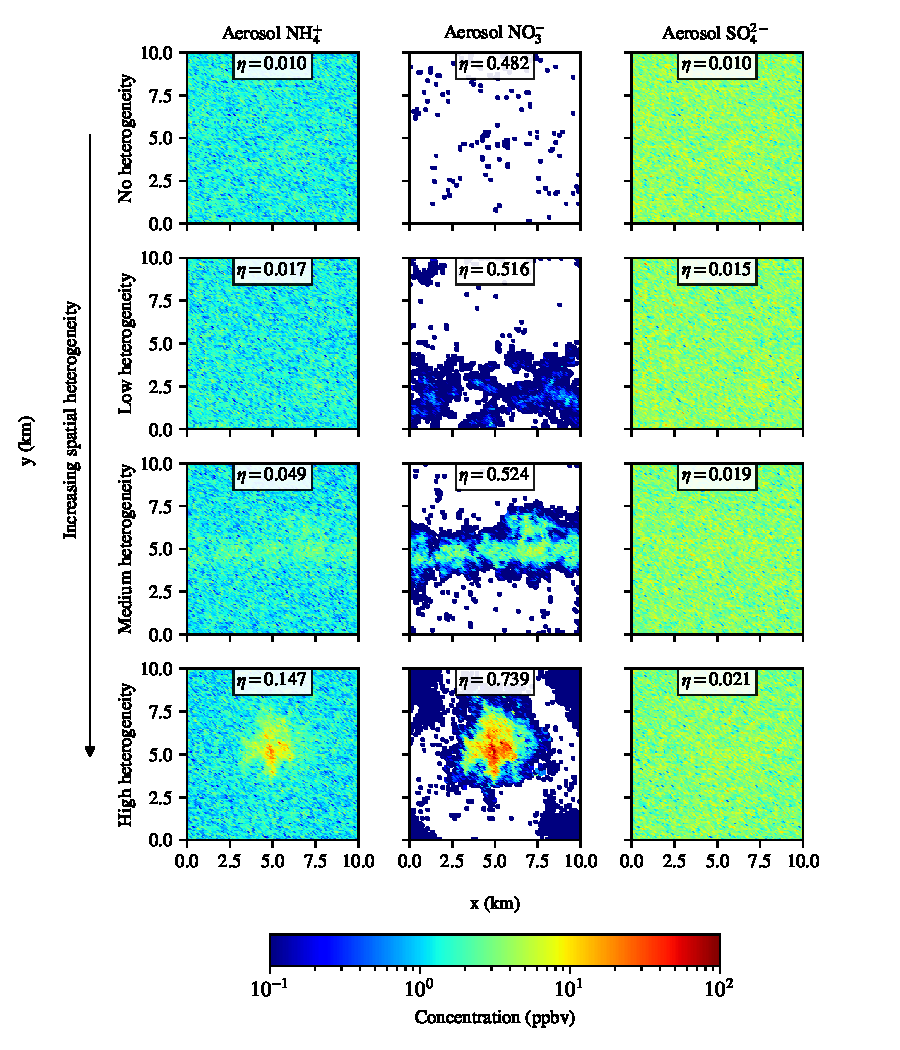
\includegraphics[]{figures/aerosol-SNA-spatial-heterogeneity-time36-z45.pdf}
	\caption{Cross sections in the x-y plane of aerosol species
          NH$_4^+$ (left column), NO$_3^-$ (center column), and
          SO$_4^{2-}$ (right column). Cross sections are shown at a
          height of approximately $z\approx900$~m and at
          $t=6$~h. Coloring indicates the concentration of aerosol
          species in parts per billion by volume. The value of the
          spatial heterogeneity metric $\eta$ is displayed alongside
          each cross section plot.}
	\label{fig:aero-cross-sec}
\end{figure} 

Figure \ref{fig:aero-cross-sec} shows cross sections of aerosol
ammonium, nitrate, and sulfate in the upper boundary layer
($z\approx900$~m) at $t=6$~h. The spatial distribution of ammonium and
nitrate closely follow the emissions plume, indicating that ammonium
nitrate formation occurs where ammonia and nitric acid are
abundant. In these regions, excess gas phase concentrations drive
partitioning into the aerosol phase. Further out from the emissions
plume, ammonium and nitrate concentrations quickly fall off as the
equilibrium condition shifts to the gas phase.

In contrast, sulfate is more uniformly distributed across all
scenarios, resulting in lower spatial heterogeneity for Scenario~3
($\eta=0.021$) compared to ammonium ($\eta = 0.142$) and nitrate
($\eta=0.739$).  This is due to the extremely low volatility of
sulfuric acid which remains almost entirely in the aerosol phase as
sulfate regardless of proximity to the emissions plume. Unlike ammonia
and nitric acid, which partition dynamically between the gas and
aerosol phase, sulfate does not re-enter the gas phase. Consequently,
the spatial distribution of aerosol species is determined by their
volatility, with less volatile species exhibiting more uniform
distributions, while higher volatility species remain clustered near
plumes with high concentrations of corresponding gas phase precursors.
Given the sensitivity of nitrate formation to the spatial
heterogeneity of emissions, nitrate levels are extremely low in the
uniform base case, with most grid cells containing no
nitrate. Occasionally, some grid cells may briefly contain particles
with nitrate. For the spatial heterogeneity metric, this is akin to
the point source scenario. As a result, the spatial heterogeneity of
nitrate for the uniform base case appears higher ($\eta=0.513$) than
the value of $\eta$ for ammonium and sulfate ($\eta=0.010$ and
$\eta=0.011$, respectively).

\begin{figure}[!h]
	\centering
	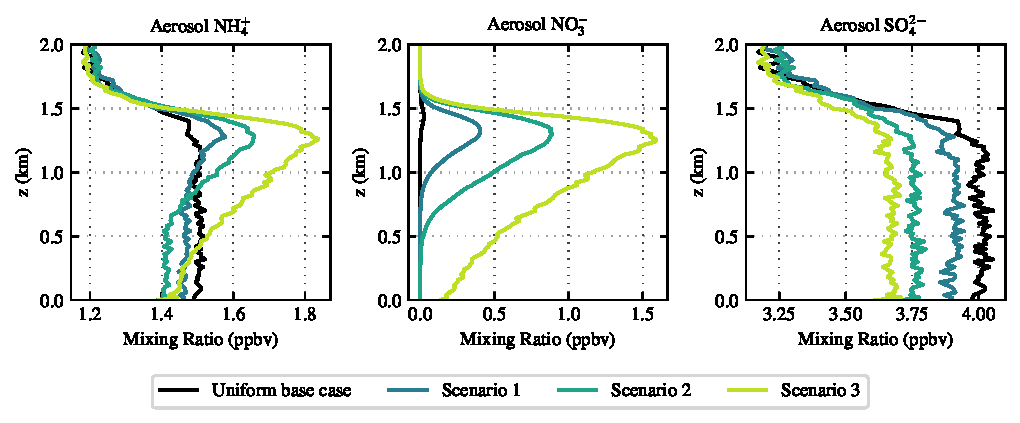
\includegraphics[]{figures/aerosol-SNA-vertical-profiles-time36.pdf}
	\caption{Vertical profiles of aerosol species NH$_4^+$ (left),
          NO$_3^-$ (center), and SO$_4^{2-}$ (right) at $t=6$ h and in
          parts per billion by volume (ppbv). For each compound, the
          mean value is displayed at each vertical level. Values for
          the uniform base case are shown as a solid black line while
          emissions scenarios 1--3 are shown as colored solid lines.}
	\label{fig:vertical-profile-SNA}
\end{figure} 

Figure \ref{fig:vertical-profile-SNA} shows vertical profiles of
aerosol ammonium (NH$_4^+$), nitrate (NO$_3^-$), and sulfate
(SO$_4^{2-}$) for each emissions scenario. These profiles represent
the average concentrations within each vertical level at the end of
each simulation ($t=6$ h).

Sulfate concentrations are nearly uniform within the boundary layer
and rapidly decrease above the entrainment zone due to limited mixing
between the free troposphere and boundary layer. Sulfate
concentrations decrease as the emissions spatial heterogeneity
increases. Production of sulfate relies on the oxidation of SO$_2$ by
OH. Within the high concentration environment of the emissions plume,
many reactive gas phase compounds including volatile organic compounds
(VOCs) complete alongside SO$_2$ for oxidation. With OH rapidly
depleted near the emissions plume, oxidation of SO$_2$ into
H$_2$SO$_4$ proceeds at a slower rate, reducing sulfate formation. OH
from outside the emissions plume is not mixed fast enough into the
plume to restore its concentration (see Figure
\ref{fig:gas-cross-sec}). Thus, segregation of OH and SO$_2$ alters
sulfate production due to the spatial heterogeneity of emissions.

Both ammonium and nitrate concentrations increase with height in the
boundary layer due to the strong temperature dependence of ammonium
nitrate formation. Nitrate availability depends on the presence of
free ammonia, i.e., ammonia not already neutralizing
sulfate as ammonium sulfate. In the lowest 500~m of the boundary
layer, the concentration of NH$_4^+$ decreases under high emissions
spatial heterogeneity due to lower
sulfate concentrations at higher emissions spatial
heterogeneity.  

At higher altitudes ($z\sim1.2$~km), ammonium nitrate formation is
enhanced for scenarios with high emissions spatial
heterogeneity. Under these conditions, the concentration of free
ammonia increases due to lower sulfate levels, allowing neutralization
of more nitric acid.  In the uniform base case, little nitrate is
formed due to the overall lower concentrations of nitric acid and
ammonia, pushing their equilibrium partitioning to the gas phase. This
indicates the strong dependence of nitrate concentrations on the
composition of the aerosol and the level of emissions spatial
heterogeneity.


\begin{figure}[!h]
	\centering
	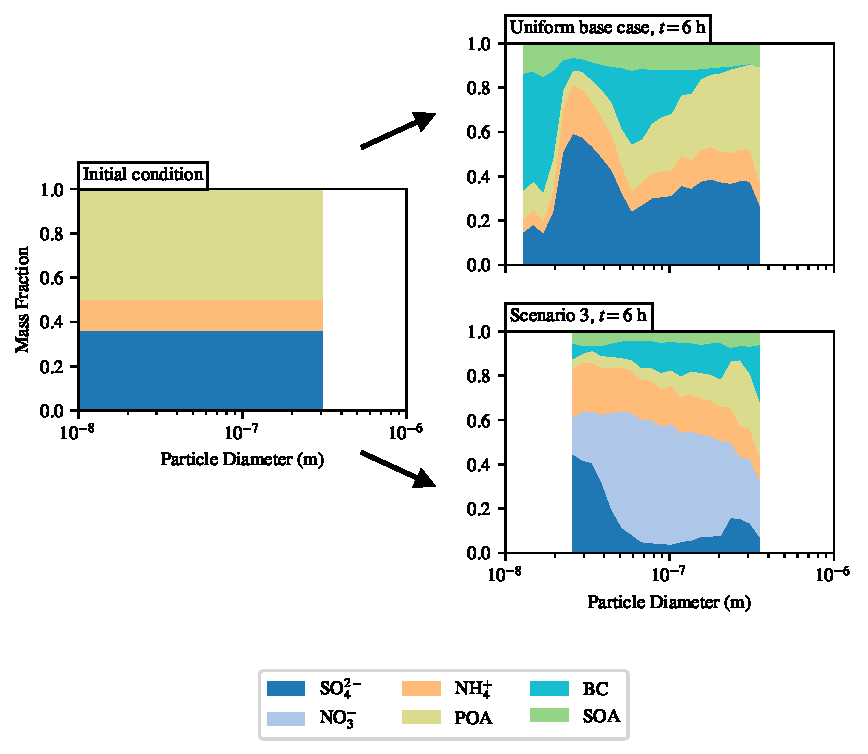
\includegraphics[]{figures/speciated-mass-frac-three-panel-z40.pdf}
	\caption{Speciated mass fraction as a function of particle
          diameter for emissions scenario extremes (uniform base case
          and Scenario~3). The initial condition is shown on the left,
          indicating that aerosol begin as an equal mixture of POA and
          ammonium sulfate. On the right, emissions scenarios with
          minimum spatial heterogeneity (top, uniform base case) and
          maximum spatial heterogeneity (bottom, Scenario~3) are shown
          after 6 hours.}
	\label{fig:speciated-mass-frac}
\end{figure} 

Figure \ref{fig:speciated-mass-frac} shows the size-resolved mass
fraction of aerosols in the upper boundary layer ($z\approx 800$ m)
for the initial condition and at the end of simulations ($t=6$ h) for
both the uniform base case and Scenario~3. After 6 hours, significant
differences in composition emerge. Under uniform emissions, particles
mainly consist of BC and primary organic aerosol (POA) along with some
sulfate. By contrast, particles in Scenario~3 are dominated by
nitrate, ammonium, and sulfate, which together comprise 50--80\% of
aerosol mass.

The CCN activity of particles in the size range of 50--100 nm is
largely governed by their composition. Figure
\ref{fig:speciated-mass-frac} indicates that, for the uniform base
case, particles in this size range are primarily composed of low
hygroscopicity compounds, including BC and POA. In Scenario~3, the
dominant presence of sulfate, nitrate, and ammonium increases particle
hygroscopicity.  This suggests that particles in the size range of
50--100 nm, whose CCN activity depends on aerosol composition, exhibit
greater hygroscopicity under high emissions spatial heterogeneity,
allowing them to activate at lower
supersaturations. We show this is indeed the case
by evaluating changes in the 2-dimensional number distribution 
$n(D_p, \kappa)$ as a function of particle diameter $D_p$ and particle
hygroscopicity parameter $\kappa$.


\begin{figure}[!t]
	\centering
	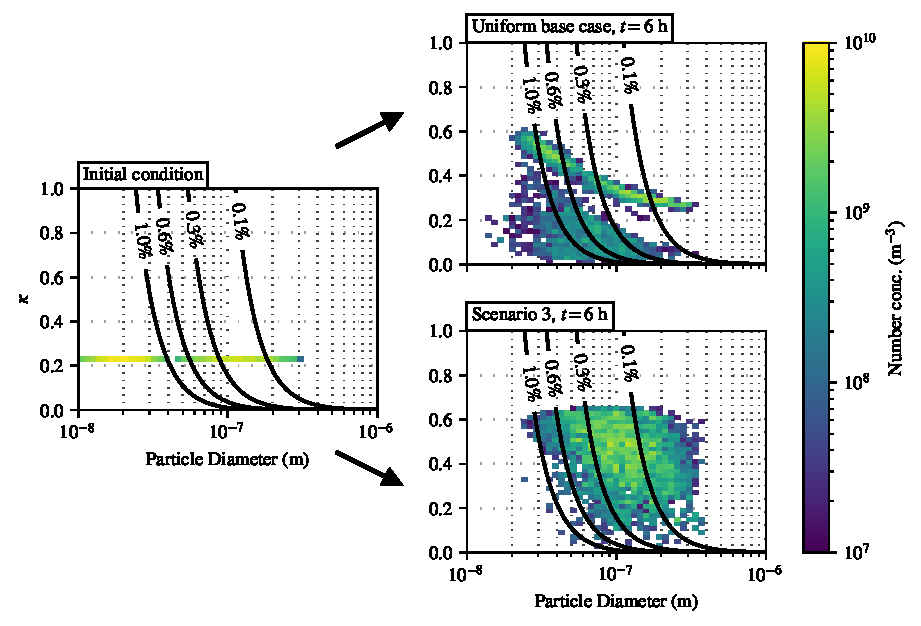
\includegraphics[]{figures/2d-kappa-dist-three-panel-z40.pdf}
	\caption{2-dimensional number distributions $n(D_p, \kappa)$ for emissions scenario extremes. The initial condition is shown on the left, indicating that all aerosol begin as internally mixed particles with uniform $\kappa$. On the right, emissions scenarios with minimum spatial heterogeneity (top, uniform base case) and maximum spatial heterogeneity (bottom, Scenario~3) are shown after 6 hours. Cell coloring indicates particle number concentration. Black solid contours indicate supersaturation in $\%$. Particles to the right of a contour line activate at the indicated supersaturation.}
	\label{fig:kappa-dist}
\end{figure} 

Figure \ref{fig:kappa-dist} shows 2-dimensional number distributions
$n(D_p, \kappa)$ for emissions scenario extremes. Each distribution
was sampled in the upper boundary layer ($z\approx 800$~m) at the
beginning and end of simulations. Initially, all particles possess the
same composition and thus the same hygroscopicity.  The right panel
compares distributions at $t=6$~h for the uniform base case and
Scenario~3.

In the uniform base case, two distinct particle groups emerge: one
with low $\kappa$ values (0--0.3), corresponding to primary
carbonaceous aerosols that have not undergone significant aging, and
another with higher $\kappa$ (0.3--0.6), representing particles that
have undergone coagulation and gas-particle partitioning. The latter
group is enriched in sulfate as seen in Figure
\ref{fig:speciated-mass-frac}.

Under Scenario~3, particles exhibit significantly higher
hygroscopicities. For instance, the hygroscopicity of particles with
diameter of 100 nm exceeds $\kappa>0.6$ (indicating highly hygroscopic
particles), whereas $\kappa$ only reaches up to 0.4 in the uniform
base case. As suggested in discussing the link between aerosol 
composition and CCN activity for particles in the size range of 
$D_p\sim50\text{--}100$~nm, this indicates that spatially heterogeneous 
emissions indeed lower the critical supersaturation of such particles, 
enhancing their CCN activity.

Differences in the $\kappa$ distributions between the uniform base
case and Scenario~3 stem from the interaction between emissions
spatial heterogeneity and sub-grid scale aerosol processes. Enhanced
coagulation in emissions plumes reduces Aitken mode particle
concentrations, explaining the absence of a low-$\kappa$ carbonaceous
aerosol group in Scenario~3. Furthermore, spatially heterogeneous
emissions promote gas-particle partitioning, increasing particle
hygroscopicity. In particular, higher concentrations of nitric acid
and ammonia near spatially heterogeneous emissions plumes drive the
equilibrium condition into the aerosol phase, raising the
concentration of ammonium nitrate alongside particle hygroscopicity.


\subsection{CCN activity}\label{sec:ccn-activ}

\begin{figure}[!h]
	\centering
	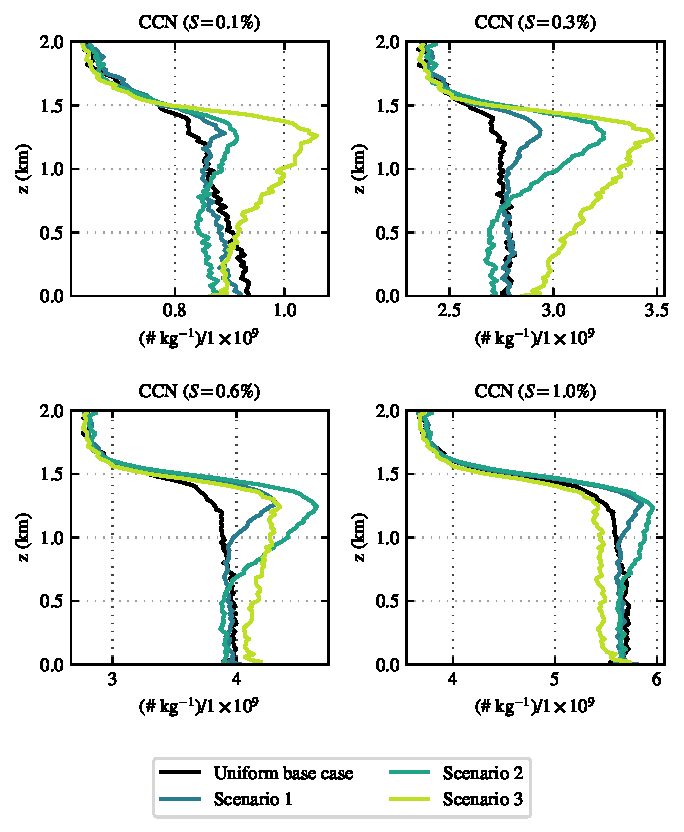
\includegraphics[]{figures/aerosol-ccn-vertical-profiles-time36.pdf}
	\caption{Vertical profiles for CCN concentrations activating
          at supersaturations $S=0.1, 0.3, 0.6, 1.0\%$ and at $t=6$
          h. Concentrations are displayed in number of CCN per
          kilogram of dry air and are scaled by a factor of
          $1\cdot10^{-9}$. Values for the uniform base case are shown
          as a solid black line while emissions scenarios 1--3 are
          shown as colored solid lines.}
	\label{fig:ccn-vertical-prof}
\end{figure} 

Figure \ref{fig:ccn-vertical-prof} shows vertical profiles of the CCN 
number per kilogram of dry air for 
supersaturations $S$ ranging from $S=0.1\%$ to $S=1.0\%$ across
different emissions scenario. Since the ambient relative humidity (RH)
never exceeds 100\% in these simulations, the reported CCN
concentrations represent the number of particles that would activate
if RH were raised to the specified supersaturation.

As noted earlier, emissions spatial heterogeneity influences aerosol
processes such as coagulation and gas-particle partitioning, altering
the particle number, size, composition, and hygroscopicity. In turn, these
modifications impact CCN activity, though the dominant
processes and their effects vary with supersaturation.

At lower supersaturations ($S=0.1\text{--}0.3\%$), CCN concentrations 
increases with emissions spatial heterogeneity
in the upper boundary layer. This is due to enhanced formation of
ammonium nitrate in the cooler, sulfate-poor environment, which
increases activation of ultrafine particles in the range of 50--100 nm
due to the high hygroscopicity of ammonium nitrate.

At higher supersaturations ($S=0.6\text{--}1.0\%$), CCN concentrations
still increase in the upper boundary layer for scenarios with lower
spatial heterogeneity, however, in Scenario~3, CCN concentrations
decrease, particularly at $S=1.0\%$, where CCN concentrations drop
below all other scenarios including the uniform base case. This is due to 
enhanced coagulation in highly heterogeneous
emissions scenarios which reduces the number of smaller particles that would
otherwise activate at high supersaturations.  Therefore, at
sufficiently high supersaturation and emissions spatial heterogeneity,
the negative effect on CCN concentration due to coagulation offsets
the positive effect of gas-particle partitioning of hygroscopic
material.

\begin{figure}[!h]
	\centering
	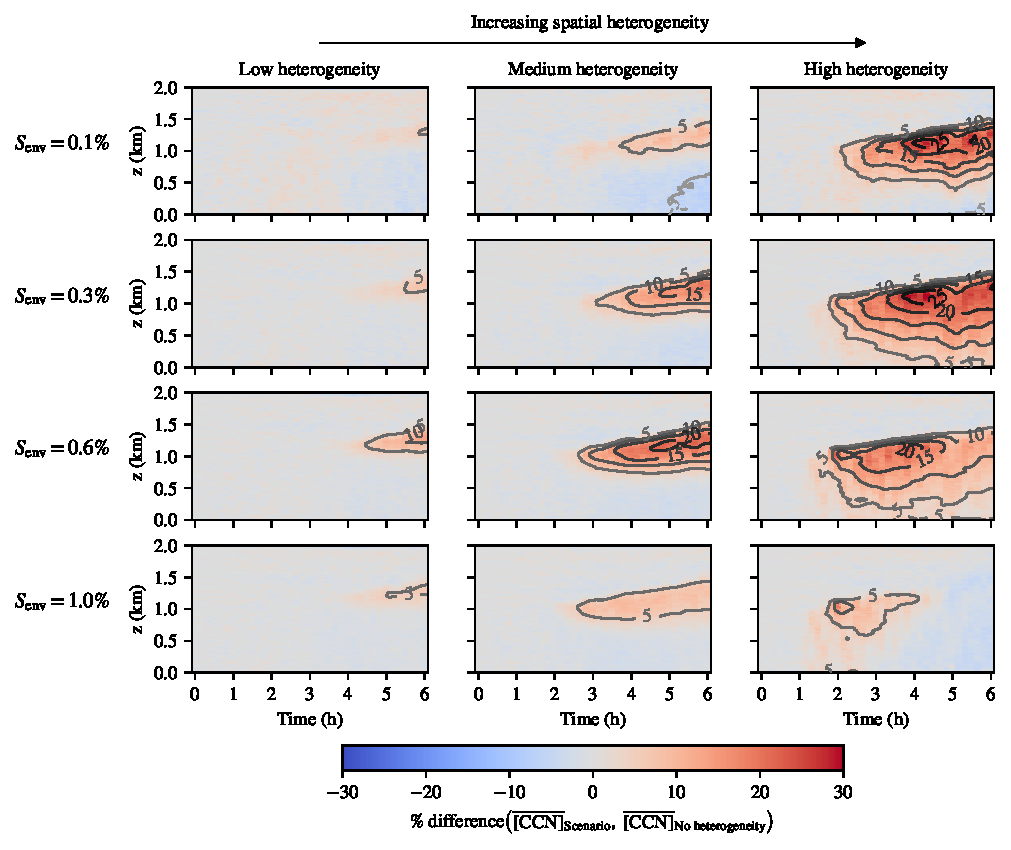
\includegraphics[]{figures/height-time-ccn-pdiff-multi-scenario.pdf}
	\caption{Time-height plots for the percent difference between
          CCN concentrations in the uniform base case and each
          emissions scenario and supersaturation level. Scenarios are
          organized by column. The supersaturation of CCN activation
          is organized by row. Red indicates an increase in CCN
          relative to the base case while blue indicates a reduction
          in CCN concentrations. Contour lines indicating regions of
          constant percent difference are drawn on each panel in
          increments of 5\%.}
	\label{fig:time-height-ccn-pdiff}
\end{figure} 

Figure \ref{fig:time-height-ccn-pdiff} illustrates the temporal and
vertical evolution of the percent difference between the CCN
concentrations relative to the uniform base case for each scenario and
supersaturation level. The percent difference is calculated as
\begin{equation}
    \% \text{ difference} = 100\times\left(\frac{\overline{[\text{CCN}]}(t, z, S)_{\text{Scenario}} - \overline{[\text{CCN}]}(t, z, S)_{\text{Base case}}}{\overline{[\text{CCN}]}(t, z, S)_{\text{Base case}}}\right),
\end{equation}
where $\overline{[\text{CCN}]}(t, z,S)$ is the horizontally averaged
concentration of CCN at time $t$ and vertical level $z$ that activate
at supersaturation $S$.

The greatest increase in CCN concentration relative to the uniform
base case occurs for Scenario~3 at $S=0.3\%$, where CCN concentrations
increase by more than 25\% through $t=6$~h. At both high
supersaturations and high emissions spatial heterogeneity, the
reduction in CCN activity due to enhanced coagulation becomes evident
after $t\approx5$~h.  Across all scenarios, CCN concentrations
increase most near the top of the boundary layer. This region grows
with time due to boundary layer development. Notably, shallow cumuli
and stratiform clouds tend to form in the upper boundary layer. This
suggests that emissions spatial heterogeneity could enhance clould
albedo through the first indirect effect.

%\begin{figure}[!t]
%	\centering
%	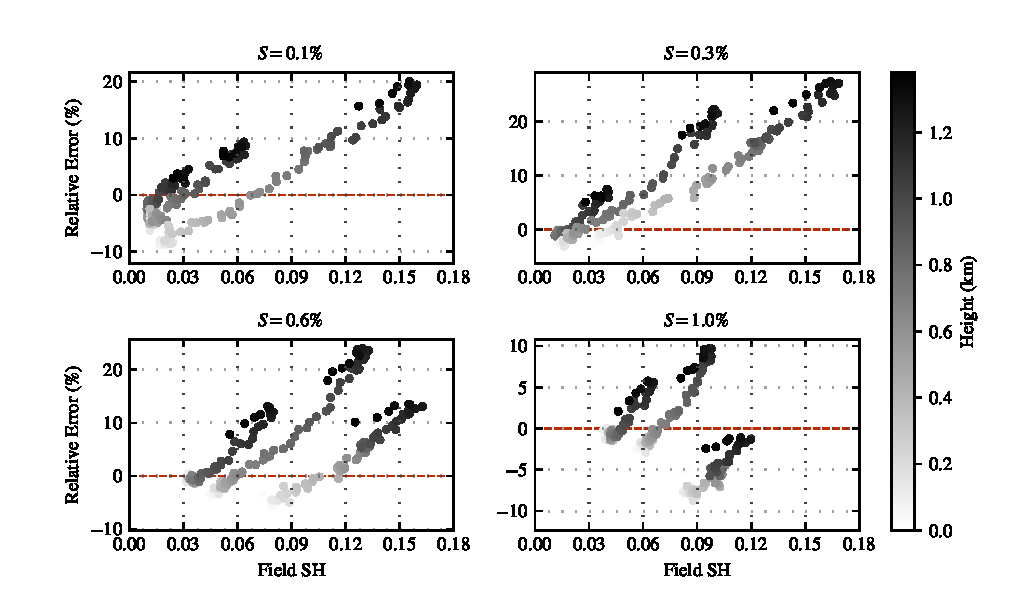
\includegraphics[]{figures/4panel-ccn-rel-err-vs-sh.pdf}
%	\caption{Make absolute value plots and remove coloring by height20}
%	%\label{fig:transport-vs-aerosol-model}
%\end{figure} 


\subsection{Influence of ammonia on aerosol composition and CCN activity}\label{sec:influence-ammonia}

To further explore the role of ammonia in CCN activity under spatially
heterogeneous emissions, we conducted additional simulations for the
uniform base case and Scenario~3, setting total ammonium
(NH$_{3\text{, gas}} + $NH$_{4\text{, aerosol}}$) to zero. Correspondingly, 
emissions of NH$_3$ were set to zero to ensure that total ammonium remains
zero throughout each simulation.

\begin{figure}[!h]
	\centering
	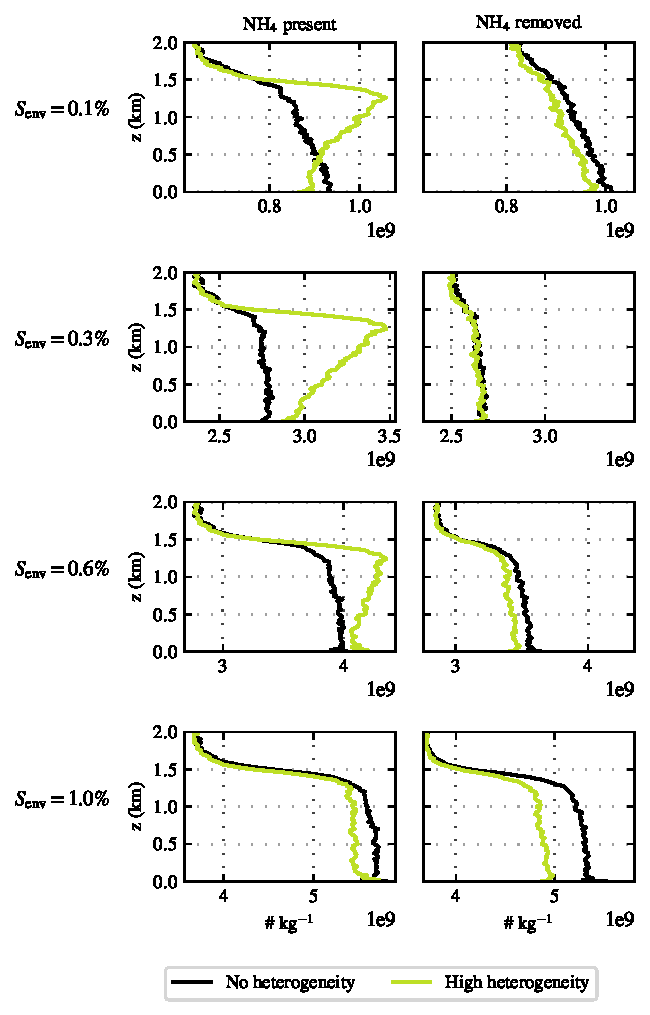
\includegraphics[]{figures/aerosol-ccn-vertical-profiles-no-nh4-cases-time36.pdf}
	\caption{Vertical profiles for CCN concentrations in
          ammonia-free simulations that activate at supersaturations
          $S=0.1, 0.3, 0.6, 1.0\%$ and at $t=6$ h. Concentrations are
          displayed in number of CCN per kilogram of dry air and are
          scaled by a factor of $1\cdot10^{-9}$. Profiles for
          scenarios with ammonia are shown as solid lines while
          scenarios without ammonia are displayed as dashed lines for
          the uniform base case (black) and Scenario~3
          (chartreuse).}
	\label{fig:ccn-vertical-profile-no-ammonia}
\end{figure}

Figure \ref{fig:ccn-vertical-profile-no-ammonia} shows vertical
profiles of CCN mixing ratios at $t=6$ h for supersaturations ranging
from $S=0.1\%$ to $S=1.0\%$. Without ammonia, CCN concentrations at
each supersaturation level agree much more closely between the uniform
base case and Scenario~3. The peak of CCN concentrations in the upper
boundary layer and at lower supersaturations, previously observed in
Scenario~3, disappears entirely. This underscores the crucial role of
ammonium nitrate formation in modulating CCN concentrations under
spatially heterogeneous emissions, especially at lower
supersaturations.

At higher supersaturations ($S=1.0\%$), scenarion 3 exhibits lower CCN
concentrations than its ammonia-free uniform base case
counterpart. This further confirms that, in the absence of
ammonia-driven gas-particle partitioning, coagulation-induced particle
loss dominates, leading to an overall reduction in the concentration of 
CCN. The similarity in CCN profiles between the ammonia-free
cases of Scenario~3 and the uniform base case, apart from a slight
(~5\%) downward shift in Scenario~3 due to enhanced coagulation,
underscores the competing influences of emissions spatial
heterogeneity on aerosol-cloud interactions.

\conclusions  %% \conclusions[modified heading if necessary]

% work this text in somewhere in the conclusion
%Past research has established a clear link between the spatial heterogeneity of both gas phase and aerosol emissions, the processes by which the aerosol age, and their resulting climate-relevant properties including CCN activity which contribute to indirect radiative forcing. Simultaneously, there exists large uncertainty in the radiative forcing due to aerosols which results in part from the coarse representation of both aerosols and their transport in global scale models and their coupling with non-linear processes that occur at the sub-grid scale such as coagulation and turbulence-chemistry interactions. Past research has led to the development of detailed aerosol model treatments and transport representations, however there has yet to be a direct coupling between particle-resolved aerosol models and turbulence-resolving transport models for use in quantifying the effects of emissions spatial heterogeneity on the aerosol state and CCN activity.

This study investigates the impact of spatially heterogeneous
emissions on aerosol properties, including CCN activity, in a
convective boundary layer using the particle-resolved large-eddy
simulation modeling framework, WRF-PartMC-MOSAIC-LES. This
first-of-its-kind modeling platform enables a detailed process-level
analysis of the coupling between emissions spatial heterogeneity and
concentration-dependent aerosol processes such as coagulation and
gas-particle partitioning. To assess these interactions, we compare
multiple idealized emissions scenarios against a base case of uniform
emissions, which serves as a proxy for coarser-resolved models that
lack the ability to resolve heterogeneity of emissions.

Our results demonstrate that emissions spatial heterogeneity
significantly alters key aerosol processes. In particular, nitrate
formation increases substantially in regions of high emissions
heterogeneity due to localized enhancements in nitric acid and ammonia
concentrations near the emissions plume core. This shifts the
equilibrium favoring ammonium nitrate formation in the aerosol
phase. In turn, the volatility of aerosol species is coupled with the
spatial heterogeneity of emissions and precursor species.
Low-volatility compounds such as sulfate are more spatially
homogeneous due to their tendency to remain in the aerosol phase even
as particles are transported away from the emissions plume.
Additionally, higher emissions heterogeneity intensifies coagulation,
accelerating particle growth and modifying the size distribution of
aerosols.

These aerosol process changes have downstream effects on CCN
activity. Notably, the influence of emissions spatial heterogeneity on
CCN concentrations is goverend by competing effects of coagulation and
gas-particle partitioning. Coagulation removes smaller particles that
would otherwise activate at high supersaturations, resulting in a
decrease in CCN activity at high supersaturations for scenarios with
high emissions spatial heterogeneity. Conversely, coagulation is not
as efficient at removing larger particles that activate at lower
supersaturations. In contrast, gas-particle partitioning results in an
increase of highly hygroscopic compounds such as ammonium nitrate
under high emissions spatial heterogeneity. As a result, CCN activity
at lower supersaturations ($S = 0.3\mbox{–-}0.6\%$) increases by up to
25\% in the upper boundary layer for emissions scenarios with high
spatial heterogeneity.

The sensitivity of CCN activity to emissions spatial heterogeneity is highly
influenced by the aerosol and gas phase composition. Given the key
contribution of ammonium nitrate formation in elevating CCN activity
under highly spatially heterogeneous scenarios, removing ammonia
weakens---or in some cases reverses---the trend between emissions
spatial heterogeneity and CCN concentrations.

This has important implcations for global climate models, where 
nitrate formation is often simplified by assuming equilibrium partitioning 
or omitted altogether. Our findings highlight the necessity of accurately 
representing nitrate in global climate models due to the strong coupling 
between emissions spatial heterogeneity, aerosol composition, and 
CCN activity. As model resolution continues to improve, advancing the 
representation of aerosol chemistry will be critical to capturing the full impact of
emissions spatial heterogeneity on cloud microphysics and climate.

\textcolor{red}{I rephrased the next paragraph a bit according to our
  discussion.}  This study uses highly idealized emission patterns, in
which all sources are spatially collocated, and a limited set of
aerosol types under fixed meteorological conditions. While our results
show that aerosol composition mediates the impact of spatial
heterogeneity on properties such as CCN activity, future work should
expand this analysis to more realistic scenarios. In particular, it
will be important to examine cases with spatially separated emission
sources, a broader diversity of primary aerosol types, and a range of
meteorological conditions that influence transport, mixing, and cloud
formation. Such studies will help determine the generality of our
findings across different geographic settings, including urban,
agricultural, and remote regions.

%\begin{itemize}
%\item Limitations and future work
%\end{itemize}

%% The following commands are for the statements about the availability of data sets and/or software code corresponding to the manuscript.
%% It is strongly recommended to make use of these sections in case data sets and/or software code have been part of your research the article is based on.

\codeavailability{TEXT} %% use this section when having only software code available


\dataavailability{TEXT} %% use this section when having only data sets available


\codedataavailability{TEXT} %% use this section when having data sets and software code available


\sampleavailability{TEXT} %% use this section when having geoscientific samples available


\videosupplement{TEXT} %% use this section when having video supplements available


\appendix
\section{}    %% Appendix A

\subsection{}     %% Appendix A1, A2, etc.


\noappendix       %% use this to mark the end of the appendix section. Otherwise the figures might be numbered incorrectly (e.g. 10 instead of 1).

%% Regarding figures and tables in appendices, the following two options are possible depending on your general handling of figures and tables in the manuscript environment:

%% Option 1: If you sorted all figures and tables into the sections of the text, please also sort the appendix figures and appendix tables into the respective appendix sections.
%% They will be correctly named automatically.

%% Option 2: If you put all figures after the reference list, please insert appendix tables and figures after the normal tables and figures.
%% To rename them correctly to A1, A2, etc., please add the following commands in front of them:

\appendixfigures  %% needs to be added in front of appendix figures

\appendixtables   %% needs to be added in front of appendix tables

%% Please add \clearpage between each table and/or figure. Further guidelines on figures and tables can be found below.



\authorcontribution{TEXT} %% this section is mandatory

\competinginterests{TEXT} %% this section is mandatory even if you declare that no competing interests are present

\disclaimer{TEXT} %% optional section

\begin{acknowledgements}
TEXT
\end{acknowledgements}




%% REFERENCES

%% The reference list is compiled as follows:

%\begin{thebibliography}{}

%\bibitem[AUTHOR(YEAR)]{LABEL1}
%REFERENCE 1

%\bibitem[AUTHOR(YEAR)]{LABEL2}
%REFERENCE 2

%\end{thebibliography}

%% Since the Copernicus LaTeX package includes the BibTeX style file copernicus.bst,
%% authors experienced with BibTeX only have to include the following two lines:
%%
\bibliographystyle{copernicus}
\bibliography{refs_sh_impacts_aerosol.bib}
%%
%% URLs and DOIs can be entered in your BibTeX file as:
%%
%% URL = {http://www.xyz.org/~jones/idx_g.htm}
%% DOI = {10.5194/xyz}


%% LITERATURE CITATIONS
%%
%% command                        & example result
%% \citet{jones90}|               & Jones et al. (1990)
%% \citep{jones90}|               & (Jones et al., 1990)
%% \citep{jones90,jones93}|       & (Jones et al., 1990, 1993)
%% \citep[p.~32]{jones90}|        & (Jones et al., 1990, p.~32)
%% \citep[e.g.,][]{jones90}|      & (e.g., Jones et al., 1990)
%% \citep[e.g.,][p.~32]{jones90}| & (e.g., Jones et al., 1990, p.~32)
%% \citeauthor{jones90}|          & Jones et al.
%% \citeyear{jones90}|            & 1990



%% FIGURES

%% When figures and tables are placed at the end of the MS (article in one-column style), please add \clearpage
%% between bibliography and first table and/or figure as well as between each table and/or figure.

% The figure files should be labelled correctly with Arabic numerals (e.g. fig01.jpg, fig02.png).


%% ONE-COLUMN FIGURES

%%f
%\begin{figure}[t]
%\includegraphics[width=8.3cm]{FILE NAME}
%\caption{TEXT}
%\end{figure}
%
%%% TWO-COLUMN FIGURES
%
%%f
%\begin{figure*}[t]
%\includegraphics[width=12cm]{FILE NAME}
%\caption{TEXT}
%\end{figure*}
%
%
%%% TABLES
%%%
%%% The different columns must be seperated with a & command and should
%%% end with \\ to identify the column brake.
%
%%% ONE-COLUMN TABLE
%
%%t
%\begin{table}[t]
%\caption{TEXT}
%\begin{tabular}{column = lcr}
%\tophline
%
%\middlehline
%
%\bottomhline
%\end{tabular}
%\belowtable{} % Table Footnotes
%\end{table}
%
%%% TWO-COLUMN TABLE
%
%%t
%\begin{table*}[t]
%\caption{TEXT}
%\begin{tabular}{column = lcr}
%\tophline
%
%\middlehline
%
%\bottomhline
%\end{tabular}
%\belowtable{} % Table Footnotes
%\end{table*}
%
%%% LANDSCAPE TABLE
%
%%t
%\begin{sidewaystable*}[t]
%\caption{TEXT}
%\begin{tabular}{column = lcr}
%\tophline
%
%\middlehline
%
%\bottomhline
%\end{tabular}
%\belowtable{} % Table Footnotes
%\end{sidewaystable*}
%
%
%%% MATHEMATICAL EXPRESSIONS
%
%%% All papers typeset by Copernicus Publications follow the math typesetting regulations
%%% given by the IUPAC Green Book (IUPAC: Quantities, Units and Symbols in Physical Chemistry,
%%% 2nd Edn., Blackwell Science, available at: http://old.iupac.org/publications/books/gbook/green_book_2ed.pdf, 1993).
%%%
%%% Physical quantities/variables are typeset in italic font (t for time, T for Temperature)
%%% Indices which are not defined are typeset in italic font (x, y, z, a, b, c)
%%% Items/objects which are defined are typeset in roman font (Car A, Car B)
%%% Descriptions/specifications which are defined by itself are typeset in roman font (abs, rel, ref, tot, net, ice)
%%% Abbreviations from 2 letters are typeset in roman font (RH, LAI)
%%% Vectors are identified in bold italic font using \vec{x}
%%% Matrices are identified in bold roman font
%%% Multiplication signs are typeset using the LaTeX commands \times (for vector products, grids, and exponential notations) or \cdot
%%% The character * should not be applied as mutliplication sign
%
%
%%% EQUATIONS
%
%%% Single-row equation
%
%\begin{equation}
%
%\end{equation}
%
%%% Multiline equation
%
%\begin{align}
%& 3 + 5 = 8\\
%& 3 + 5 = 8\\
%& 3 + 5 = 8
%\end{align}
%
%
%%% MATRICES
%
%\begin{matrix}
%x & y & z\\
%x & y & z\\
%x & y & z\\
%\end{matrix}
%
%
%%% ALGORITHM
%
%\begin{algorithm}
%\caption{...}
%\label{a1}
%\begin{algorithmic}
%...
%\end{algorithmic}
%\end{algorithm}
%
%
%%% CHEMICAL FORMULAS AND REACTIONS
%
%%% For formulas embedded in the text, please use \chem{}
%
%%% The reaction environment creates labels including the letter R, i.e. (R1), (R2), etc.
%
%\begin{reaction}
%%% \rightarrow should be used for normal (one-way) chemical reactions
%%% \rightleftharpoons should be used for equilibria
%%% \leftrightarrow should be used for resonance structures
%\end{reaction}
%
%
%%% PHYSICAL UNITS
%%%
%%% Please use \unit{} and apply the exponential notation


\end{document}



% Old Intro

Aerosols are known to impose a net negative radiative forcing, however considerable uncertainty persists in the representation of radiative forcing due to aerosol-cloud interactions (ACI) \citep{ipcc_report_2021}. Advancements in computing power have allowed modelers to investigate key contributing factors which alter the intensity of radiative forcing due to ACI such as spatial resolution \citep{ma_how_2015}. Simultaneously, improvements in computational power have advanced the representation of aerosols in climate models through inclusion of more complex chemical mechanisms \citep{zaveri_development_2021} and detailed aerosol treatments such as the Community Aerosol and Radiation Model for Atmospheres (CARMA) , which is a 40 bin sectional model used by the Community Earth System Model 2 (CESM2) \citep{tilmes_description_2023} and has shown improvements in representing aerosol properties when compared to the 4 bin Modal Aerosol Model (MAM4). While these two key structural components to models---the treatment of aerosols and the effect of spatial resolution---have improved representation of aerosols and their radiative forcing, these aspects have yet to be explored in tandem to investigate the role of spatial heterogeneities typically below the grid scale of current climate models alongside detailed aerosol treatments in modifying the depiction of climate-relevant aerosol properties key to ACI such as cloud condensation nuclei (CCN) activity.

Aerosol concentrations and properties vary at scales ranging from global and regional variability down to local and hyper-local spatial heterogeneity near emissions sources. Numerous lines of evidence point to the multi-scale spatial variability of aerosols. At the global-scale, satellite remote sensing with platforms such as MODIS have shown large-scale variability in bulk quantities including aerosol optical depth (\hl{cite}). At the regional scale, field campaigns have shown considerable variability in aerosol properties such as concentration, size distributions, CCN concentrations, and composition \citep{fast_using_2022}. Local in-situ measurements of aerosol properties are highly dependent on proximity to emissions sources such as vehicular combustion, and past studies have shown that aerosol abundance and composition vary on the scale of 10s to 100s of meters downwind of sources due to non-linear processes such as coagulation \citep{zhu_study_2002}. Indeed, hyper-local heterogeneity in aerosol properties frustrates traditional comparison between point-source measurements and grid-cell averaged model quantities, and distributed measurement networks such as the Portable Optical Particle Spectrometer network in the Southern Great Plains (POPSnet-SGP) campaign aim to elucidate climate model uncertainty associated with sub-grid scale aerosol spatial heterogeneity \citep{asher_novel_2022}. 

\hl{Could also note that aerosol heterogeneities are coupled to other sources of heterogeneity by inducing feedbacks on, for instance, heterogeneous surface properties such as radiative heating and soil moisture, which have been shown to induce secondary circulations (Lee et al. 2019, Tian et al. 2022)}

Aerosol-aware climate models typically contain a sub-model which governs the aerosol representation and associated processes. Given computational constraints, the aerosol treatment is often highly simplified with regard to aerosol compositional diversity. For instance, E3SM uses the modal aerosol model MAM4 which contains four lognormally distributed modes \citep{golaz_doe_2022}. Such a treatment constrains the diversity of the aerosol population to four internally-mixed modes (i.e., all particles within a mode are compositionally identical). As a result, modal and sectional aerosol treatments underrepresent the true compositional complexity of an aerosol population in which each particle ages independently. Particle-resolved aerosol models allow representation of the full compositional diversity of an aerosol population via a set of computational particles which are allowed to compositionally vary and age independently. Particle resolved models such as the Particle Monte Carlo model (PartMC) have been used extensively to investigate the sensitivity of CCN activity to the composition of emitted aerosol particles \citep{fierce_when_2013}, aging timescales due to condensation and coagulation for carbonaceous CCN \citep{fierce_explaining_2015}, and the sensitivity of CCN estimates to mixing state (i.e., the compositional diversity within and across aerosols) \citep{ching_metrics_2017}. Furthermore, given that a particle-resolved model can fully represent aerosol composition space, PartMC has been used to estimate error in CCN activity for coarser aerosol treatments by comparing depicted CCN concentrations against compositionally-averaged output reminiscent of a sectional or modal model \citep{zaveri_particle-resolved_2010, ching_metrics_2017}. Furthermore, direct comparison of CCN activity depicted by PartMC and MAM4 has shown considerable divergence, especially in polluted regions where high rates of coagulation and gas-particle partitioning amplify model disagreement \citep{fierce_quantifying_2024}. 

In addition to the treatment of aerosols, the depiction of spatial heterogeneity---including that of surface properties, emissions of gas phase species and primary aerosol, and heterogeneous distributions of their resulting plumes---influences particle aging and associated properties including CCN activity. Present aerosol-aware models at regional and global scales possess insufficient resolution to capture the full spatial heterogeneity of aerosols and the emissions of primary aerosols and gas phase precursors. In turn, these models depict artificially dilute and uniform concentrations within grid cells. This alters the representation of concentration-dependent, non-linear aerosol processes such as coagulation and gas particle partitioning. Past studies have shown that climate-relevant aerosol properties such as aerosol optical properties \citep{gustafson_jr_downscaling_2011} and CCN activity \citep{weigum_effect_2016} are highly sensitive to the model’s grid resolution with a large contribution of sub-grid scale variability resulting from the spatially varying pattern of emissions \citep{qian_investigation_2010}. 

%Given large uncertainties in the effective radiative forcing resulting from aerosol-cloud interactions \citep{ipcc_report_2021}, constraining model estimates of CCN activity remains an important focus. 

Past studies evaluating the sub-grid variability of aerosol properties often compare outputs from models with coarse resolution typical of global climate models ($\sim 50$--$100$ km) against higher resolution model outputs with resolution on the order of $\sim 1$--$10$ km 
\citep{qian_investigation_2010, gustafson_jr_downscaling_2011, weigum_effect_2016, crippa_impact_2017, lin_quantification_2017}. While such improvements in resolution better resolve heterogeneities in emissions, there still exists considerable unresolved spatial heterogeneity in the sub-kilometer scale. In addition, such modeling studies do not explicitly resolve the scales of turbulent transport in the boundary layer, instead fully parameterizing turbulence via Reynolds-averaged Navier Stokes. 

Furthermore, these models use simplified representations of aerosols such as modal or sectional treatments. Comparing these aerosol treatments against particle-resolved models which represent the broad compositional complexity of aerosols, past studies have shown that simplified aerosol representations impact modeled aerosol properties including CCN activity \citep{zaveri_particle-resolved_2010, ching_metrics_2017, fierce_quantifying_2024}.

The evolution of emission plumes containing gas phase compounds and aerosols is highly dependent on turbulent mixing at fine spatial scales and the proximity of reactive species. A considerable body of literature has investigated the role of turbulence-chemistry interactions and chemical segregation on gas phase reactions in the planetary boundary layer via the use of large-eddy simulations (LES). \citet{brasseur_segregation_2023} review recent applications of LES to investigate chemical segregation and turbulence chemistry interactions in a variety of spatially heterogeneous geographic regions. Past studies tend to focus on the oxidation of highly reactive volatile organic compounds (VOCs) such as isoprene and have shown that spatially heterogeneous emissions contribute to the chemical segregation between reactive gas phase species in the boundary layer \citep{ouwersloot_segregation_2011, kaser_chemistry-turbulence_2015}. Note, however, that these studies do not model aerosols, although the coupling between the gas phase and aerosols through gas-particle partitioning suggests chemical segregation due to the spatial heterogeneity of emissions likely influences the aerosol state. 
%\hl{Also note Jeff Pierce's work}


Recently, numerous turbulence-resolving frameworks have been coupled to aerosol models including the use of the Sectional Aerosol model for Large Scale Applications (SALSA) \citep{kokkola_salsa_2008} alongside UCLALES \citep{tonttila_uclalessalsa_2017} and the Parallelized Large-Eddy Simulation Model (PALM) \citep{kurppa_implementation_2019} as well as the coupling between the modal model M7 \citep{vignati_m7_2004} and the Dutch Atmospheric Large-Eddy Simulation model (DALES) \citep{de_bruine_explicit_2019}.
%Both models have been used to investigate aerosol-cloud interactions and compare model outputs against field campaign measurements. 
Although these models have high-resolution transport schemes, they each possess relatively coarse-resolution aerosol treatments. For instance, UCLALES-SALSA uses a 10-bin sectional treatment while DALES implements a modified version of the seven-mode M7 model to allow two additional hydrometeor modes. To our knowledge, no aerosol-aware transport model has yet to leverage a high-resolution particle resolved aerosol treatment alongside turbulence resolving transport frameworks such as LES. 

%\hl{I don't really consider LES models that couple microphysics schemes (such as the microphysics scheme of Feingold 1996) since they simply parameterize the aerosols and number of CCN but there are more of such models in existence than purely aerosol-aware LES.}

%\begin{itemize}
%\item SAM + modal Aitken mode aerosol microphysics scheme (Wyant et al. 2022)
%\item PNNL-LES + 2D binned microphysics (Ovchinnikov and Easter 2010)
%\end{itemize}

The aim of this work is to conduct a process-level analysis of the the complex coupling between the spatial heterogeneity of surface emissions (including both gas compounds and primary aerosol), aerosol aging processes, and the resulting impact on aerosol properties including CCN activity via a set of first-of-a-kind particle-resolved LES. This establishes a high resolution aerosol-transport model framework in both explicit representation of turbulent transport as well as aerosol composition, properties, and aging.

This paper is organized in the following manner. Section 2 presents the modeling framework used in this study, WRF-PartMC-MOSAIC-LES, alongside a description of numerous emissions scenarios ranging in spatial heterogeneity. Section 3 discusses results of simulation runs, and a description of changes to the aerosol size distribution, composition, hygroscopicity, and CCN activity across emissions scenarios are discussed. We conclude with remarks on the implications of this study, limitations stemming from its idealized nature, and future work. 
